\section{1174051 - Evietania Charis Sujadi}
\subsection{Teori}
\begin{enumerate}
\item Definisi, sejarah, dan juga pengembangan Kecerdasan Buatan
\subitem Definisi kecerdasan diciptakan oleh pengetahuan yang dapat membuat komputer untuk kecerdasan manusia terkait dengan penangkapan, pemodelan, dan penyimpanan kecerdasan manusia dalam suatu sistem teknologi. Contohnya adalah melakukan analisis penalti untuk menarik kesimpulan atau menerjemahkan kelemahan atau memutuskan dari satu bahasa ke bahasa lain.
\subitem Sejarah dan perkembangan intelijen terjadi pada musim panas 1956 menerima seminar tentang AI di Darmouth College. Seminar dihadiri oleh para ahli komputer dan membahas potensi komputer dalam pengaduan kecerdasan manusia. Namun, perkembangan yang sudah sering terjadi sejak LISP diciptakan, yaitu kecerdasan buatan yang dibuat pada tahun 1960 oleh John McCarthy. Istilah kecerdasan buatan atau Inteligensi Buatan diambil dari Marvin Minsky dari MIT. Dia menulis sebuah makalah ilmiah yang berjudul Steps to Artificial Intelligence, Institute for Proceedings of Radio Engineers 49, Januari 1961. 
\item  Definisi supervised learning, klasifikasi, regresi, dan unsupervised learning. Data set, training set dan testing set. 
\subitem Supervised learning merupakan sebuah pendekatan dimana sudah terdapat data yang dilatih, dan terdapat variable yang ditargetkan sehingga tujuan dari pendekatan ini adalah mengkelompokan suatu data ke data yang sudah ada. Sedangkan unsupervised learning tidak memiliki data latih, sehingga dari data yang ada, kita mengelompokan data tersebut menjadi 2 bagian atau 3 bagian dan seterusnya.
\subitem Klasifikasi adalah salah satu topik utama dalam data mining atau machine learning. Klasifikasi yaitu suatu pengelompokan data dimana data yang digunakan tersebut mempunyai kelas label atau target.
\subitem Regresi adalah Supervised learning tidak hanya mempelajari classifier, tetapi juga mempelajari fungsi yang dapat memprediksi suatu nilai numerik. Contoh, ketika diberi foto seseorang, kita ingin memprediksi umur, tinggi, dan berat orang yang ada pada foto tersebut.
\subitem Data set adalah cabang aplikasi dari Artificial Intelligence/Kecerdasan Buatan yang fokus pada pengembangan sebuah sistem yang mampu belajar sendiri tanpa harus berulang kali di program oleh manusia.
\subitem Training set yaitu jika pasangan objek, dan kelas yang menunjuk pada objek tersebut adalah suatu contoh yang telah diberi label akan menghasilkan suatu algoritma pembelajaran.
\subitem Tujuan dari set tes adalah untuk menentukan sejauh mana classifier berhasil membuat klasifikasi dengan benar
\end{enumerate}
\subsection{Instalasi}
\begin{enumerate}
\item {Instalasi Library Scikit}
Masuk pada windows lalu search "conda" , setelah itu akan muncul Anaconda prompt. lalu ketikkan conda install scikit-learn
\begin{figure}[ht]
\centering
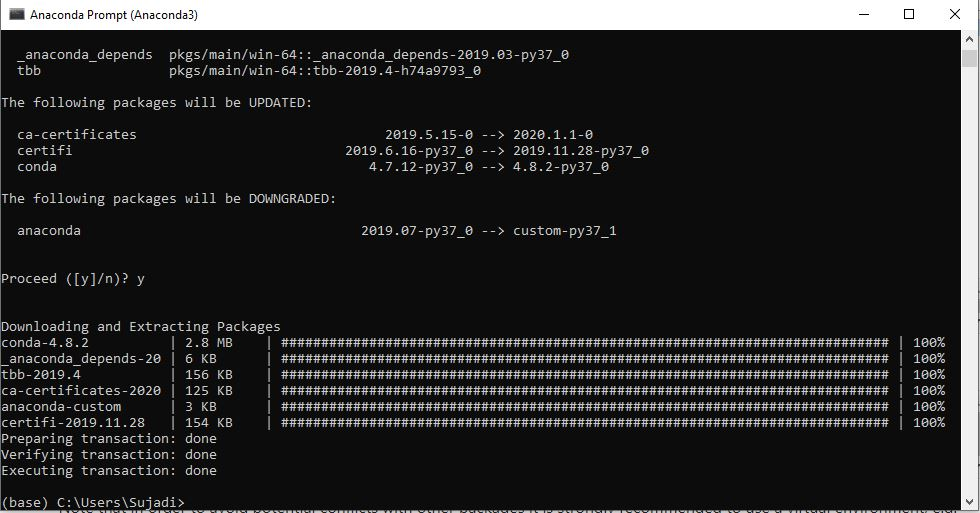
\includegraphics[scale=0.5]{figures/1174051/1/1.JPG}
\caption{Installasi}
\label{contoh}
\end{figure}
\begin{figure}[H]
\centering
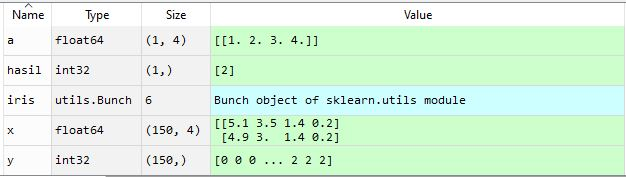
\includegraphics[width=4cm]{figures/1174051/1/2.JPG}
\caption{Isi Variabel Explorer}
\end{figure}
\item Mencoba loading an example dataset
\hfill\break
\lstinputlisting[firstline=8, lastline=12]{src/1174051/1/1174051.py}
\item Mencoba Learning dan predicting
\hfill\break
\lstinputlisting[firstline=14, lastline=24]{src/1174051/1/1174051.py}
\item Mencoba Model Persistence
\hfill\break
\lstinputlisting[firstline=26, lastline=36]{src/1174051/1/1174051.py}
\item Mencoba Conventions
\hfill\break
\lstinputlisting[firstline=38, lastline=50]{src/1174051/1/1174051.py}
\end{enumerate}
\subsection{Penanganan Error}
\begin{enumerate}
\item ScreenShoot Error
\begin{figure}[H]
	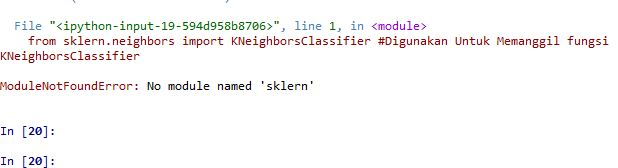
\includegraphics[width=4cm]{figures/1174051/1/error/1.JPG}
	\centering
	\caption{Import Error}
\end{figure}
\item Tuliskan Kode Error dan Jenis Error
\begin{itemize}
	\item ModuleNotFoundError
\end{itemize}
\item Cara Penangan Error
\begin{itemize}
	\item ModuleNotFoundError
	\hfill\break
	Typo pada pemanggilan sklearn
\end{itemize}
\end{enumerate}
\subsection{Bukti Tidak Plagiat}
\begin{figure}[H]
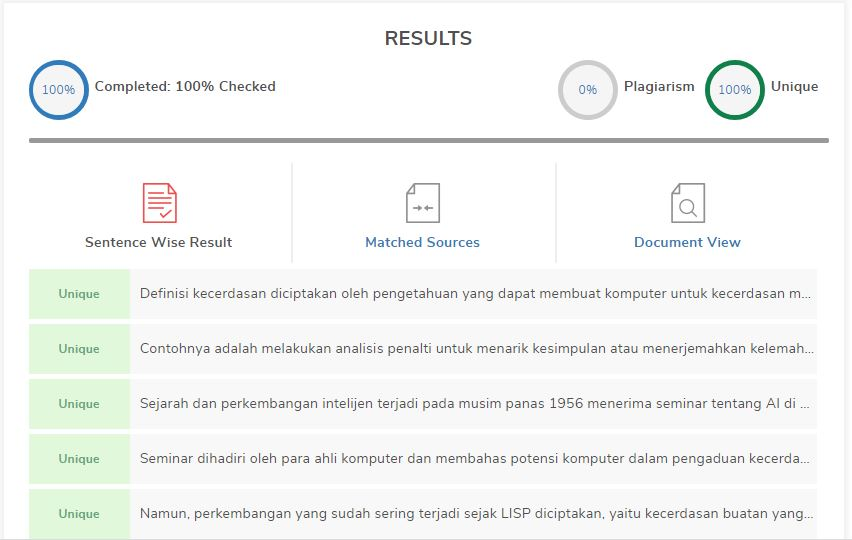
\includegraphics[width=4cm]{figures/1174051/1/plagiat/1.JPG}
\centering
\caption{Bukti Tidak Melakukan Plagiat 1}
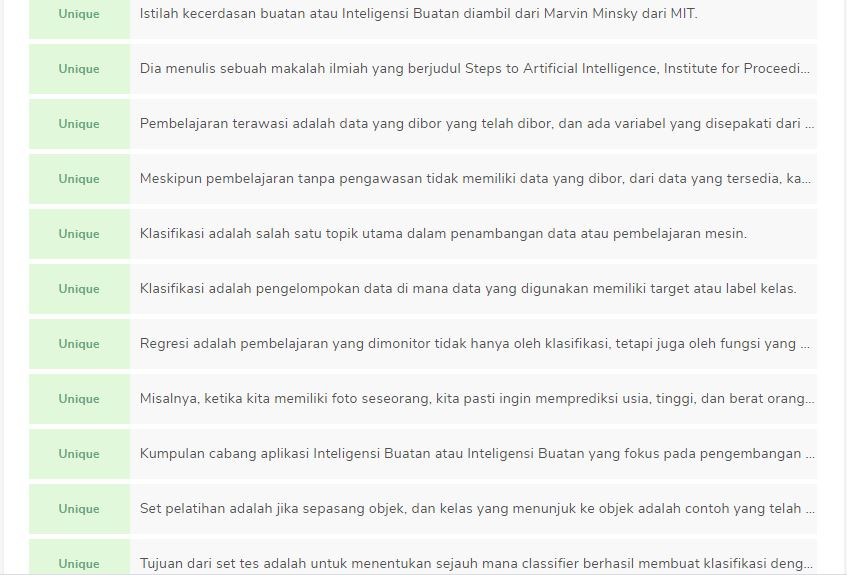
\includegraphics[width=4cm]{figures/1174051/1/plagiat/2.JPG}
\centering
\caption{Bukti Tidak Melakukan Plagiat 2}
\end{figure}